% Created 2016-08-17 Wed 14:38
\documentclass[tikz]{standalone}

\usepackage[utf8]{inputenc}
\usepackage[T1]{fontenc}

\usepackage{circledsteps}

\RequirePackage{xcolor}

%% HPI color definitions according to the design manual
% These do not exactly match the RGB values used in the Powerpoint slide master due to unknown reasons
\definecolor{hpiyellow}{RGB}{246,168,0}
\definecolor{hpiorange}{RGB}{221,97,8}
\definecolor{hpired}{RGB}{177,6,58}
\definecolor{hpigray}{RGB}{90,96,101}
\definecolor{hpiblue}{RGB}{0,122,158}


\renewcommand{\sfdefault}{neosans}
% Different font weights for neosans
\newcommand{\textl}[1]{{\fontseries{l}\selectfont #1}} % light
\newcommand{\textm}[1]{{\fontseries{m}\selectfont #1}} % medium, same as default weight
\newcommand{\textsb}[1]{{\fontseries{sb}\selectfont #1}} % semibold
\newcommand{\textmb}[1]{{\fontseries{mb}\selectfont #1}} % bold, same as \textbf
\newcommand{\texteb}[1]{{\fontseries{eb}\selectfont #1}} % extra bold
\newcommand{\textub}[1]{{\fontseries{ub}\selectfont #1}} % ultra bold

\tikzset{every picture/.style={/utils/exec={\sffamily}}}
\tikzset{flipflop RSflanke/.style={
  flipflop,
  flipflop def={t1=S, t2=C, c2=1, t3=R, t6=Q, t4={\ctikztextnot{Q}}}
}}


\tikzset{
  mechanicalSwitch/.pic={
    \coordinate (-inUp) at (135:2); 
    \coordinate (-inDown) at (235:2);
    \coordinate (-out) at (2,0);
    \coordinate (-center) at (0,0);
    
    \draw (0,0) circle [radius = 2cm];
    \draw [fill=gray!20] (0,0) circle [radius = 0.2cm];

    \draw (0, 0) -- (2, 0);
    \draw (135:.8) -- (135:2); 
    \draw (225:.8) -- (225:2); 

    \draw [fill=gray!20] (2, 0) circle [radius=0.05cm]; 
    \draw [fill=gray!20] (135:2) circle [radius=0.05cm]; 
    \draw [fill=gray!20] (225:2) circle [radius=0.05cm]; 

    
    \draw [thick] (0,0) -- (175:1.5); 

    \draw [dashed, <->, domain=135:225] plot ({cos(\x)}, {sin(\x)}); 
  },
  mechanicalSwitchClosed/.pic={
    \coordinate (-inUp) at (135:2); 
    \coordinate (-inDown) at (255:2);
    \coordinate (-out) at (2,0);
    \coordinate (-center) at (0,0);
    \draw (0,0) circle [radius = 2cm];
    \draw [fill=gray!20] (0,0) circle [radius = 0.2cm];

    \draw (0, 0) -- (2, 0);
    \draw (135:.8) -- (135:2); 
    \draw (225:.8) -- (225:2); 

    \draw [fill=gray!20] (2, 0) circle [radius=0.05cm]; 
    \draw [fill=gray!20] (135:2) circle [radius=0.05cm]; 
    \draw [fill=gray!20] (225:2) circle [radius=0.05cm]; 

    
    \draw [thick] (0,0) -- (135:2); 

    \draw [dashed, <->, domain=135:225] plot ({cos(\x)}, {sin(\x)}); 
  }
}


\usetikzlibrary{calc}
\usetikzlibrary{positioning}


\usetikzlibrary{automata}
\usetikzlibrary{arrows}       %                 ...customizing arrows


\tikzset{node distance=5cm, % Minimum distance between two nodes. Change if necessary.
  every node/.style={           align=center,
},
         every state/.style={ % Sets the properties for each state
           semithick,
           fill=gray!10},
         initial text={},     % No label on start arrow
         double distance=2pt, % Adjust appearance of accept states
         every edge/.style={  % Sets the properties for each transition
           draw, ->, 
           % ->,>=stealth’,     % Makes edges directed with bold arrowheads
           auto,
           semithick}}

\begin{document}


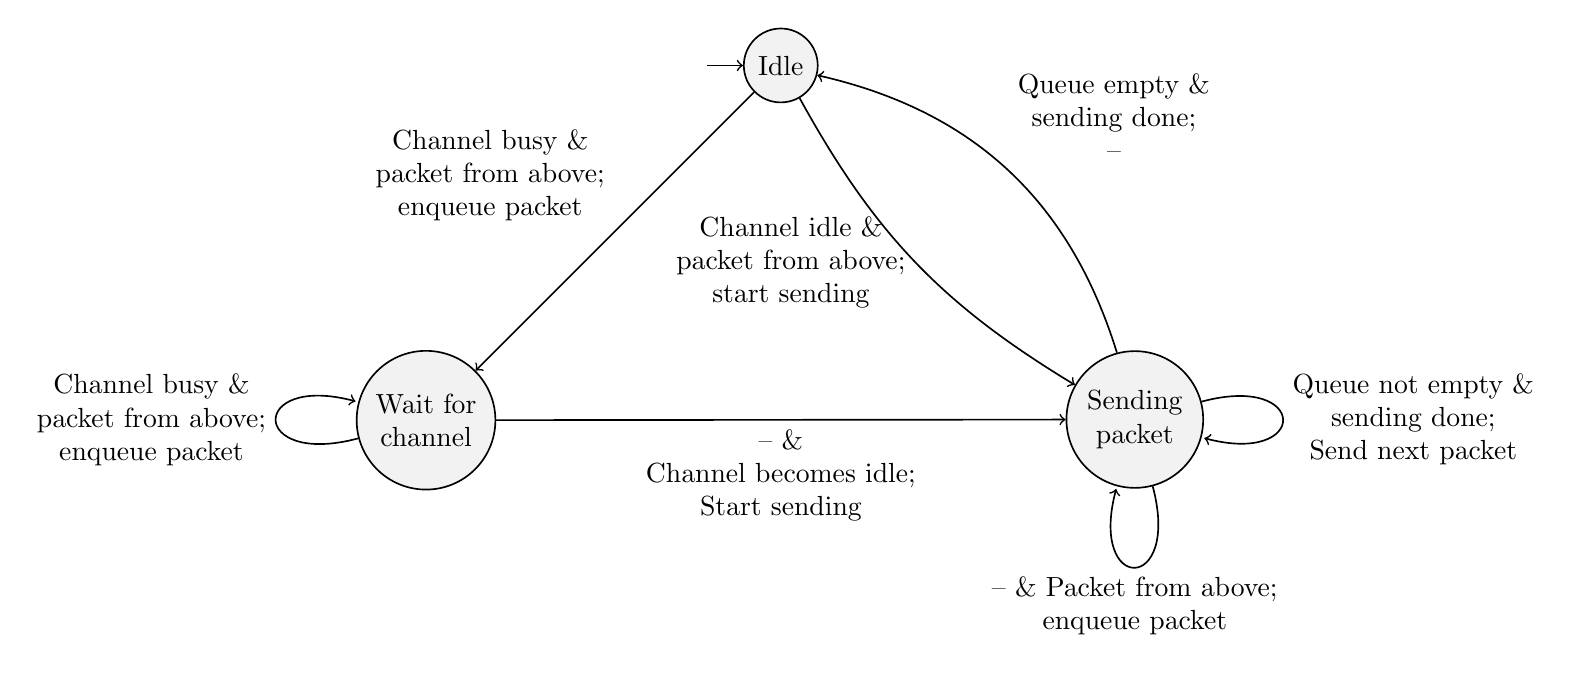
\begin{tikzpicture}
  \label{page:mac:onepersistent}
  
  \node [state, initial] (qidle) {Idle};
  \node [state, below left=of qidle] (qwait) {Wait for\\ channel};
  \node [state, below right=of qidle] (qsending) {Sending\\packet};

  \draw (qidle) edge node[above left] {Channel busy \& \\packet from above;\\enqueue packet } (qwait);
  \draw (qidle) edge[bend right=15] node[left] {Channel idle \& \\packet from above;\\start sending } (qsending);
  \draw (qwait) edge [loop left] node {Channel busy \& \\packet from above;\\enqueue packet } (qwait);
  \draw (qwait) edge node[below] {-- \& \\Channel  becomes idle;\\Start sending } (qsending);

  \draw (qsending) edge[loop right] node {Queue not empty \&\\sending done; \\Send next packet} (qsending);

  \draw (qsending)  edge [bend right=30] node[above right] {Queue empty \&\\sending done; \\--} (qidle);

  
  \draw (qsending) edge[loop below]  node[below] {-- \& Packet from above;\\enqueue packet} (qsending);

  
\end{tikzpicture}


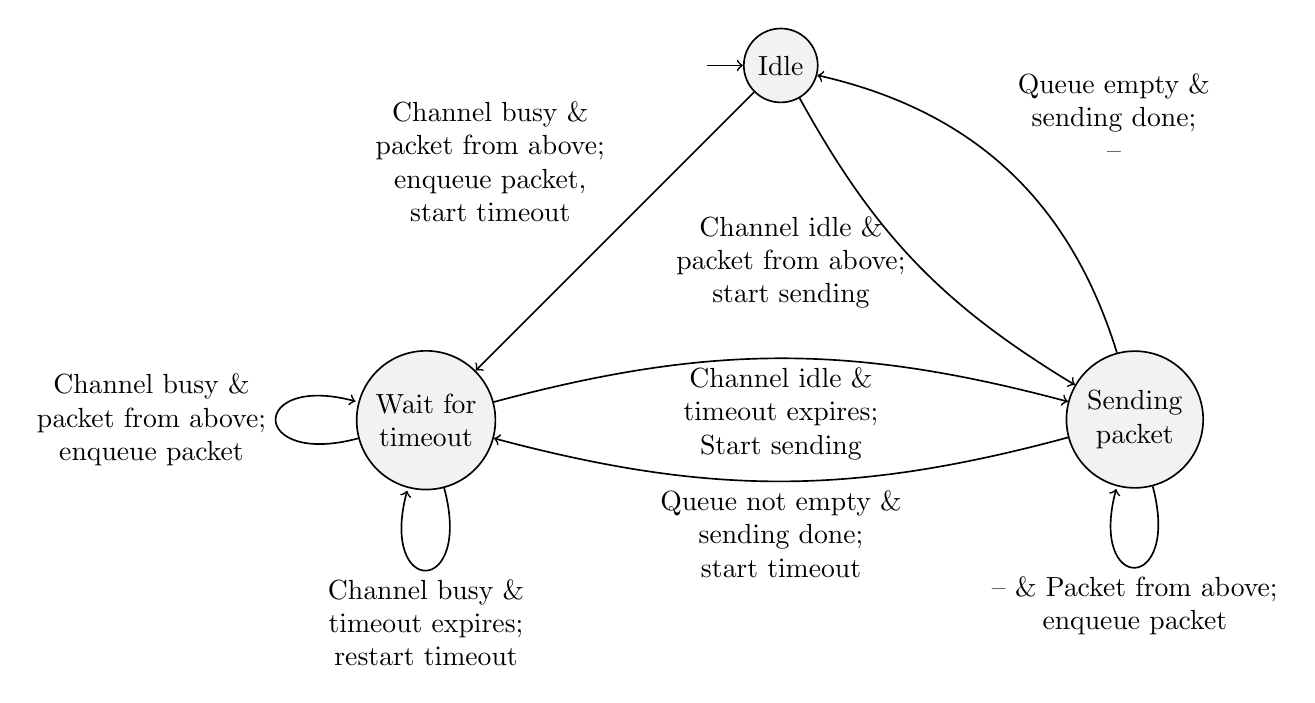
\begin{tikzpicture}
  \label{page:mac:nonpersistent}
  
  \node [state, initial] (qidle) {Idle};
  \node [state, below left=of qidle] (qwait) {Wait for\\ timeout};
  \node [state, below right=of qidle] (qsending) {Sending\\packet};

  \draw (qidle) edge node[above left] {Channel busy \& \\packet from above;\\enqueue packet,\\start timeout
  } (qwait);
  \draw (qidle) edge[bend right=15] node[left] {Channel idle \& \\packet from above;\\start sending } (qsending);
  \draw (qwait) edge [loop left] node {Channel busy \& \\packet from above;\\enqueue packet } (qwait);
  \draw (qwait) edge[bend left=15] node[below] {Channel idle \&\\timeout expires;\\Start sending } (qsending);
  \draw (qwait) edge [loop below] node[below] {Channel busy \&\\timeout expires;\\restart timeout } (qwait);

  
  \draw (qsending) edge[bend left=15] node[below] {Queue not empty \&\\sending done; \\start timeout} (qwait);

  \draw (qsending)  edge [bend right=30] node[above right] {Queue empty \&\\sending done; \\--} (qidle);

  
  \draw (qsending) edge[loop below]  node[below] {-- \& Packet from above;\\enqueue packet} (qsending);

  
\end{tikzpicture}


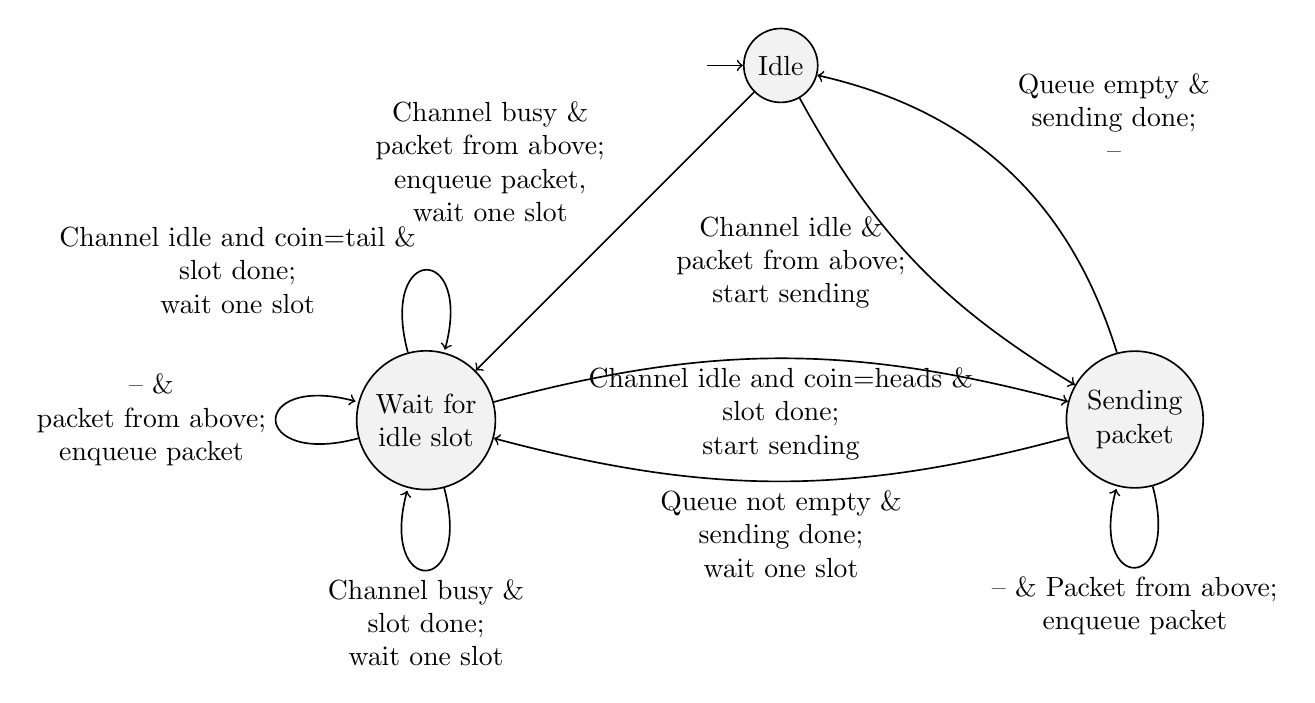
\begin{tikzpicture}
  \label{page:mac:ppersistent}
  
  \node [state, initial] (qidle) {Idle};
  \node [state, below left=of qidle] (qwait) {Wait for\\ idle slot};
  \node [state, below right=of qidle] (qsending) {Sending\\packet};

  \draw (qidle) edge node[above left] {Channel busy \& \\packet from above;\\enqueue packet,\\wait one slot
  } (qwait);
  \draw (qidle) edge[bend right=15] node[left] {Channel idle \& \\packet from above;\\start sending } (qsending);
  \draw (qwait) edge [loop left] node {-- \& \\packet from above;\\enqueue packet } (qwait);
  \draw (qwait) edge[bend left=15] node[below] {Channel idle and coin=heads \&\\slot done;\\start sending } (qsending);
  \draw (qwait) edge [loop below] node[below] {Channel busy \&\\slot done;\\wait one slot } (qwait);


  \draw (qwait) edge [loop above] node[left] {Channel idle and coin=tail \&\\slot done;\\wait one slot } (qwait);
  
  
  \draw (qsending) edge[bend left=15] node[below] {Queue not empty \&\\sending done; \\wait one slot} (qwait);

  \draw (qsending)  edge [bend right=30] node[above right] {Queue empty \&\\sending done; \\--} (qidle);

  
  \draw (qsending) edge[loop below]  node[below] {-- \& Packet from above;\\enqueue packet} (qsending);

  
\end{tikzpicture}

% \end{tikzpicture}

\end{document}